\PassOptionsToPackage{svgnames}{xcolor}
\PassOptionsToPackage{dvipsnames}{xcolor}

\documentclass[aspectratio=169]{beamer}

% Use the Turbo Vision theme
\usepackage{beamerthemeturbovision}

% Packages
\usepackage[utf8]{inputenc}
\usepackage[T1]{fontenc}
\usepackage{lmodern}
\usepackage{graphicx} % If you need to include images
\usepackage{listings}

%\definecolor{darkgreen}{RGB}{1,50,32}
%\usepackage[dvipsnames,svgnames,tikz]{xcolor}
%\usepackage{chronosys}
\usepackage{tikz}
%\usetikzlibrary{overlay-beamer-styles}
% \tikzset{
%    highlight on/.style={alt={#1{fill=red!80!black,%color=red!80!black}{fill=gray!30!white,color=gray!30!white}}},
%}

% Title Information
\title{Deploy like it's the 1980s}
\author{verMan.io}
\date{}%\date{\today}
\setbeamersize{text margin left=0pt}

\begin{document}

\begin{frame}
  \titlepage
\end{frame}

\begin{frame}{https://github.com/SamuelMarks}
    \centering
  Samuel Marks.

  \vspace{2em}
%  \begin{columns}
 %   \begin{column}{0.917\textwidth}
  \centering
%  Try it today:
  \begin{center}
    \begin{tabular}{l}
        Research fellow at Harvard Medical School / MEEI \\
        PhD from the University of Sydney \\
        >800 GitHub repos \\
        >300 of these sources not forks \\
        top 10 contributor to Keras \\
        Google Developer Expert for Machine Learning / Artificial Intelligence \\
        >13 years of software-engineering consulting experience
    \end{tabular}
  \end{center}
  
  %  \end{column}
%\end{columns}
\end{frame}

\section{Cross-platform}

\begin{frame}{More than cross-platform}
    \begin{columns}
        \begin{column}{0.5\textwidth}
           \begin{enumerate}[<+->]
                \item[0.] Docker (Linux)
                \item Linux (native)
                \item macOS
                \item Windows
                \item iOS
                \item Android
           \end{enumerate}
        \end{column}
        \begin{column}{0.5\textwidth}  %%<--- here
            \begin{enumerate}[<+->]
                \setcounter{enumi}{5}
                \item FreeBSD, OpenBSD, NetBSD
                \item HP/UX
                \item SunOS, Open Solaris, illumos
                \item z/OS
                \item DOS
                \item OS/360
            \end{enumerate}
        \end{column}
    \end{columns}
\end{frame}

\section{Cross-platform}

\begin{frame}{More than Docker}
    \begin{enumerate}
        \item[0.] Docker
    \end{enumerate}
\end{frame}

\begin{frame}{More than Docker}
    \centering
    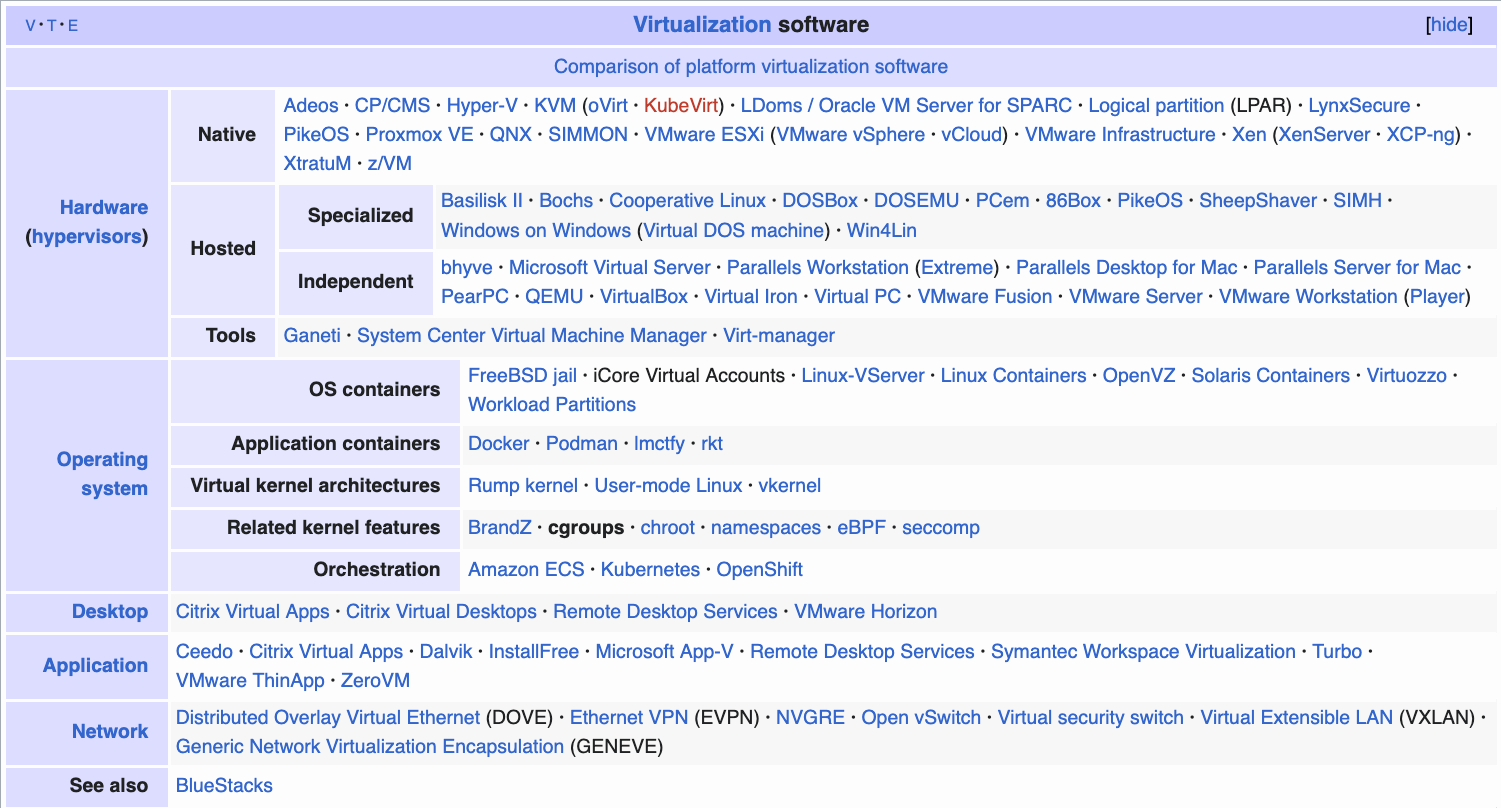
\includegraphics[width=\columnwidth]{images/virt.png}
\end{frame}

\section{Multicloud}

\begin{frame}{More than multicloud}
    \begin{columns}
        \begin{column}{0.3\textwidth}
           \begin{enumerate}[<+->]
                \setcounter{enumi}{-1}
                \item Amazon Web Services (AWS)
                \item Microsoft Azure
                \item Google Cloud
                \item IBM Cloud
                \item Alibaba Cloud Elastic Compute Service (ECS)
                \item Aurora Compute
                \item Microsoft Azure (ARM)
                \item cloudscale.ch
                \item CloudSigma
                \item Apache CloudStack
           \end{enumerate}
        \end{column}
        \begin{column}{0.3\textwidth}  %%<--- here
            \begin{enumerate}[<+->]
                \setcounter{enumi}{9}
                \item DigitalOcean
                \item Dimension Data (NTT Ltd.)
                \item Exoscale
                \item Gandi.net
                \item gridscale
                \item Ikoula
                \item Internet Solutions
                \item Kamatera
                \item libvirt
                \item Maxihost
                \item Nimbus
                \item NTT America
            \end{enumerate}
        \end{column}
        \begin{column}{0.3\textwidth}  %%<--- here
            \begin{enumerate}[<+->]
                \setcounter{enumi}{21}
                \item NTT Communications Cloud Infrastructure Services
                \item OnApp
                \item OpenStack
                \item Outscale
                \item Outscale Inc.
                \item Outscale SAS
                \item OVHcloud
                \item Rackspace
                \item Scaleway
                \item UpCloud
                \item VMware vCloud
                \item Vultr
            \end{enumerate}
        \end{column}
    \end{columns}
\end{frame}

\section{Windows and Panels}

\begin{frame}{More than open-source}
    \begin{columns}
        \begin{column}{0.5\textwidth}
  \begin{tvWindow}[License]
    \begin{center}
    public domain
    \end{center}
  \end{tvWindow}
\end{column}
\end{columns}
\end{frame}

\section{Website}
\begin{frame}{Website}
    \centering
    \Large
    \href{https://verMan.io}{https://verMan.io}
\end{frame}

\section{Features}

\begin{frame}{Unique Value Proposition}
        \begin{columns}
            \begin{column}{0.5\textwidth}
        
  \begin{tvWindow}[UVP]
    \begin{itemize}[<+->]
      \item 1-click deploy
      \item 2-click multicloud deploy
      \item Cross-platform
      \item Documentation generation
      \item Cloud / host agnostic
    \end{itemize}
  \end{tvWindow}
\end{column}
\end{columns}
\end{frame}


% \begin{frame}{Market / competition}
%     \begin{columns}
%         \begin{column}{0.617\textwidth}
    
% \begin{itemize}[<+->]
%     \item Docker\textemdash{}who \textbf{raised \$530M}\textemdash{}is roughly a direct competitor, that verMan optionally integrates with
%     \item Hashicorp\textemdash{}who \textbf{raised \$349M}\textemdash{}where verMan would particularly benefit its Vagrant and Packer
%     \item Ansible\textemdash{}who IBM \textbf{acquired for \$150M}\textemdash{}alongside Puppet, Chef, Salt, \&etc. would benefit from verMan
% \end{itemize}
% \end{column}
% \end{columns}
% \end{frame}

\begin{frame}{Revenue opportunities}
    \begin{columns}
        \begin{column}{0.617\textwidth}
    
\begin{itemize}[<+->]
    \item create a new lift-and-shift software-engineering consultancy (to/fro mainframes and clouds)
    \item selling to companies building atop kubernetes (to alternatively build atop agnostic tech);
    \item enter the as-a-Service market, or provide whitelabel as-a-Service-as-a-Service:
    \begin{itemize}[<+->]
        \item databases
        \item MLOps
        \item cpanel alternative
        \item full PaaS\textellipsis{} or similar.
    \end{itemize}
\end{itemize}
\end{column}
\end{columns}
\end{frame}

\section{Conclusion}

\begin{frame}{Roadmap}
    \begin{columns}
        \begin{column}{0.8\textwidth}
            \begin{block}{Now}
                Working version
            \end{block}
        \end{column}
    \end{columns}
    \uncover<2->{\begin{columns}
        \begin{column}{0.8\textwidth}
            \begin{block}{+1 week}
                Telemetry (OpenTelemetry linked throughout; with multiple dashboarding and metric-gathering systems)
            \end{block}
        \end{column}
    \end{columns}}
    \uncover<3->{\begin{columns}
        \begin{column}{0.8\textwidth}
            \begin{block}{+2 weeks}
                Backups; more docs; more toolchains
            \end{block}
        \end{column}
    \end{columns}}
    \uncover<4->{\begin{columns}
        \begin{column}{0.8\textwidth}
            \begin{block}{+3 weeks}
                PaaS type functionality; GitOps
            \end{block}
        \end{column}
    \end{columns}}
    \uncover<5->{\begin{columns}
        \begin{column}{0.8\textwidth}
            \begin{block}{+4 weeks}
                More databases, toolchains, servers on more OSs and distributions
            \end{block}
        \end{column}
    \end{columns}}
\end{frame}

\begin{frame}{Questions?}
    \centering
  Thank you for viewing \& attending this presentation!

  \vspace{2em}
%  \begin{columns}
 %   \begin{column}{0.917\textwidth}
  \centering
%  Try it today:
  \begin{center}
    \begin{tabular}{l}
        \href{mailto:samuel@offscale.io}{samuel@offscale.io}\\
        \href{https://github.com/SamuelMarks/libscript}{https://github.com/SamuelMarks/libscript}\\
        \href{https://github.com/verman-io}{https://github.com/verman-io}
    \end{tabular}
  \end{center}
\end{frame}

\end{document}
